\documentclass[]{article}
\newcommand{\FileDepth}{../../..}
\usepackage[letterpaper, landscape, margin=0.5cm]{geometry}
\usepackage[T1]{fontenc}
\usepackage{textcomp}%Not strictly necessary, but gives \textmu command for "micro."
\usepackage{fancyhdr}
\usepackage{amsmath}
\usepackage{amssymb}
\usepackage{graphicx}
\usepackage{xcolor}
\usepackage{tikz}
\usetikzlibrary{calc}
\usepackage[shortlabels]{enumitem}
\usepackage{multicol}
\usepackage{vwcol}
\usepackage{hyperref}
\usepackage{wrapfig}
%opening
\newcommand{\SecType}{S}
\newcommand{\Week}{4}
\title{PH 211 Studio \Week}
\author{Benjamin Bauml}
\date{Summer 2024}

\newcommand{\Purpose}{4}
\newcommand{\DefOnly}{0}

\input{\FileDepth/Formats/Assignment20240614.tex}
\usepackage[absolute]{textpos}
% This package relies on Assignment Format 2024-06-14 or later to work. It is recommended that the Purpose and DefOnly commands be given as such:
%\newcommand{\Purpose}{4}
%\newcommand{\DefOnly}{0}
% Activities need to be entered outside of the TeacherMargin and PresentSpace environments, otherwise they will be defined only locally. They can even go in the preamble.
\newenvironment{TeacherMargin}{\begin{textblock*}{10.8cm}(0.5cm,0.5cm)
\small}{\end{textblock*}
\hspace{0.1cm}}
\newenvironment{PresentSpace}{\begin{textblock*}{0.3cm}(26.85cm,9.35cm)
--
\end{textblock*}
\begin{textblock*}{15.6cm}(11.8cm,0.5cm)
\begin{Repurpose}{1}
\Large}{\end{Repurpose}
\end{textblock*}
\hspace{0.1cm}}

\newcommand{\FBDaxes}[4][2]{
	\begin{scope}[shift={(#2)},rotate=#3]
		% x-axis
		\draw[thick,->] (-#1,0) -- (#1,0);
		\node[anchor=west] at (#1,0) {$x$};
		% y-axis
		\draw[thick,->] (0,-#1) -- (0,#1);
		\node[anchor=south] at (0,#1) {$y$};
		\coordinate (#4) at (0,0);
	\end{scope}
}
\newcommand{\FBDvectorMA}[4]{
	\begin{scope}[shift={(#1)}]
		\coordinate (#4tip) at ({#2*cos(#3)},{#2*sin(#3)});
		\draw[ultra thick,blue,->] (#1) -- (#4tip);
	\end{scope}
}
\newcommand{\FBDvectorXY}[3]{
	\begin{scope}[shift={(#1)}]
		\coordinate (#3tip) at (#2);
		\draw[ultra thick,blue,->] (0,0) -- (#3tip);
	\end{scope}
}
\newcommand{\FBDdot}[1]{
	\filldraw[black] (#1) circle (3pt);
}
\newcommand{\FBDbox}[5][1]{
	\begin{scope}[shift={(#2)},rotate=#3]
		\filldraw[color=black,fill=white,thick] ({-#1/2},{#1/2}) -- ({-#1/2},{-#1/2}) -- ({#1/2},{-#1/2}) -- ({#1/2},{#1/2}) -- cycle;
		% Left side coordinates
		\coordinate (#4ltq) at ({-#1/2},{#1/4});
		\coordinate (#4lcent) at ({-#1/2},0);
		\coordinate (#4lbq) at ({-#1/2},{-#1/4});
		% right side coordinates
		\coordinate (#4rtq) at ({#1/2},{#1/4});
		\coordinate (#4rcent) at ({#1/2},0);
		\coordinate (#4rbq) at ({#1/2},{-#1/4});
		% top coordinates
		\coordinate (#4tlq) at ({-#1/4},{#1/2});
		\coordinate (#4tcent) at (0,{#1/2});
		\coordinate (#4trq) at ({#1/4},{#1/2});
		% bottom coordinates
		\coordinate (#4blq) at ({-#1/4},{-#1/2});
		\coordinate (#4bcent) at (0,{-#1/2});
		\coordinate (#4brq) at ({#1/4},{-#1/2});
		% corners
		\coordinate (#4tl) at ({-#1/2},{#1/2});
		\coordinate (#4tr) at ({#1/2},{#1/2});
		\coordinate (#4bl) at ({-#1/2},{-#1/2});
		\coordinate (#4br) at ({#1/2},{-#1/2});
		\node at (0,0) {#5};
	\end{scope}
}
%\newcommand{\MVec}[3][0]{%Creates a momentum vector of length #3 centered at #2 and rotated #1 degrees counterclockwise.
	\begin{scope}[rotate=#1,shift={(#2)}]
		\draw[->,thick] ({-#3/2},0) -- ({#3/2},0);
	\end{scope}
}
\newcommand{\MDot}[1]{%Creates a dot at #1 to represent a zero vector.
	\filldraw (#1) circle (1pt);
}
\newcommand{\MVDRows}[2][4.5]{%Creates the rows (initial, delta, final) of a momentum vector diagram. The optional argument determines the width of the table, and defaults to a good length for three columns (two objects and the total system). The non-optional argument gives a coordinate name (not displayed) to the diagram.
	\begin{scope}
		%\draw[thick] (0,5.5) -- (0,0);
		\draw[thick] (-1,4.5) -- (#1,4.5);
		\node at (-0.5,3.75) {$\vec{p}_{i}$};
		\draw[thick] (-1,3) -- (#1,3);
		\node at (-0.5,2.25) {$\Delta\vec{p}$};
		\draw[thick] (-1,1.5) -- (#1,1.5);
		\node at (-0.5,0.75) {$\vec{p}_{f}$};
		\coordinate (#2) at (0,5);
	\end{scope}
}
\newcommand{\MVDCol}[4][0.75]{%Creates a column for an object in a momentum vector diagram. The first (non-optional) argument is the coordinate name (not displayed) of the column, while the second is the displayed column header. The first argument also names the three entries down the column. The third argument anchors the column, so it should either be the coordinate name of the MVD (for the first column) or the coordinate name of the previous column. The optional argument indicates how far the center of the column should be from the previous column's edge, and defaults to 0.75.
	\begin{scope}[shift={(#4)}]
		\node at (#1,0) {#3};
		%\draw[thick] ({#1*2},0.5) -- ({#1*2},-5);
		\draw[thick] (0,0.5) -- (0,-5);
		\coordinate (#2init) at (#1,-1.25);
		\coordinate (#2delt) at (#1,-2.75);
		\coordinate (#2fin) at (#1,-4.25);
		\coordinate (#2) at ({#1*2},0);
	\end{scope}
}

%\input{\FileDepth/Activities/Activity_One/Activity_One.tex}
%\input{\FileDepth/Activities/Activity_Two/Activity_Two.tex}

\begin{document}
\begin{TeacherMargin}
\noindent One thing a teacher of mine liked to remind her students: how we perform on exams has nothing to do with our value as human beings. \\

\noindent You should discuss the feedback from your quizzes on the ungrading assignments, and you can address how they went and whether you think they were a good measure of your learning.
\end{TeacherMargin}
\begin{PresentSpace}
\begin{center}
	\huge Studio 4: Gravity and Friction \\
	\vspace{1cm}
\end{center}
\underline{Warm-Up Activity} \\
How do you feel about the quizzes? \\
\begin{center}
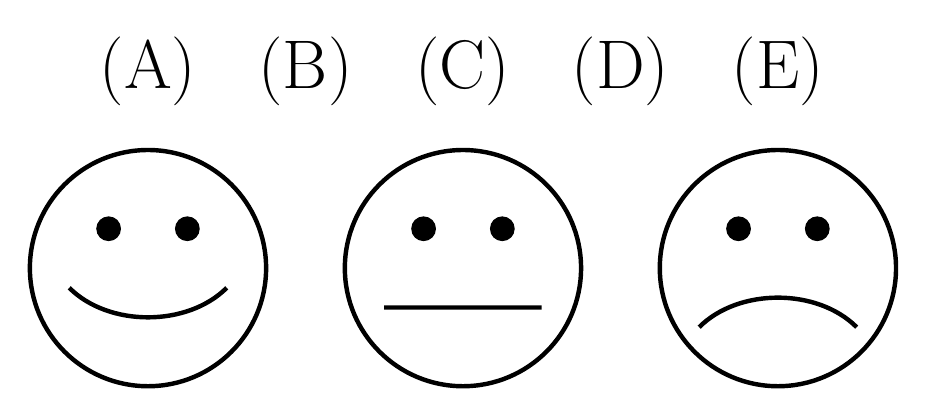
\begin{tikzpicture}
	\foreach \x in {-1,0,1}
		\draw[ultra thick] (4*\x,0) circle (1.5) (4*\x-1,-0.25*\x-0.5) .. controls (4*\x-0.5,0.25*\x-0.5) and (4*\x+0.5,0.25*\x-0.5) .. (4*\x+1,-0.25*\x-0.5);
	\foreach \x in {-1,0,1}
		\filldraw (4*\x-0.5,0.5) circle (0.15) (4*\x+0.5,0.5) circle (0.15);
	\node at (-4,2.5) {\Huge(A)};
	\node at (-2,2.5) {\Huge(B)};
	\node at (0,2.5) {\Huge(C)};
	\node at (2,2.5) {\Huge(D)};
	\node at (4,2.5) {\Huge(E)};
\end{tikzpicture}
\end{center}
\end{PresentSpace}
\newpage
\begin{TeacherMargin}

\end{TeacherMargin}
\begin{PresentSpace}
\vspace{-10pt}
\section*{(Newton's) Laws of Motion}
\vspace{-10pt}
\begin{enumerate}[(1)]
	\item An object in motion (or at rest) stays in motion (or at rest) unless a net external force acts on it.
	\item The net force on an object is equal to the object's mass times its acceleration:
	\[
	\vec{F}^{net} = m\vec{a}.
	\]
	\item If A exerts a force on B, then B exerts a force of the same magnitude on A in the opposite direction:
	\[
	\vec{F}_{AB} = -\vec{F}_{BA}.
	\]
\end{enumerate}
\end{PresentSpace}
\newpage
\begin{TeacherMargin}

\end{TeacherMargin}
\begin{PresentSpace}
\vspace{-10pt}
\section*{Types of Forces}
\vspace{-10pt}
\begin{itemize}
	\item Gravity \qquad \qquad \qquad \qquad $\vec{F}^{g}_{AB} = m_{A}\vec{g}_{B}$
	\begin{itemize}
		\item Newtonian \qquad\ $\vec{g}_{B} = G\frac{M_{B}}{r^{2}}(-\hat{r})$, $G = 6.67408\times10^{-11}\text{ N}\cdot\text{m}^{2}/\text{kg}^{2}$
		\item Near-Earth \qquad $\vec{g}_{E} = g(-\hat{y}),\ g=9.81\frac{\text{m}}{\text{s}^{2}} \approx 10\frac{\text{m}}{\text{s}^{2}}$
	\end{itemize}
	\item Normal \qquad $\vec{F}^{N}$ always $\bot$; varies in magnitude
	\item Tension \qquad $\vec{F}^{T}$ uniform (massless, inextensible rope)
	\item Spring
	\item Friction
	\begin{itemize}
		\item Static Friction \qquad $F^{sf}\leq\mu_{s}|\vec{F}^{N}|$
		\item Kinetic Friction \qquad $F^{kf}=\mu_{k}|\vec{F}^{N}|$
	\end{itemize}
\end{itemize}
\end{PresentSpace}
\newpage
\begin{TeacherMargin}
\noindent\textbf{System} \\
We don't want to pick the Earth, the elevator, and the string and ball, as then there are no external forces in that case. Instead, let us choose just the ball, which has tension from the string and a gravitational force. \\

\noindent\textbf{Assumptions}
\begin{itemize}
	\item Near-Earth gravity: $g\approx9.81\text{ m/s}^{2}$. Even if the elevator goes from the bottom to the highest point in the building, it remains near the surface of the Earth. Variation in gravitational acceleration will be negligible.
	\item Particle model. The ball will not deform or spin while hanging from a string. In particular, it probably can't spin very much with a string wrapped around it.
	\item No swinging. The problem ceases to be 1-D if the ball starts to swing side-to-side, and the swinging might affect the tension, so it is best to assume the ball hangs straight down as the elevator goes.
	\item Ideal (massless, inextensible) string. We need to assume that the mass in the string is negligible in comparison to the volleyball (which is possible for a very light string), otherwise the tension in the string will not be uniform.
\end{itemize}
\begin{center}
	\begin{tikzpicture}
		\FBDaxes{0,0}{0}{axes}
		\FBDvectorXY{axes}{0,-1}{FG}
		\node[anchor=east] at (FGtip) {$\vec{F}^{g}$};
		\FBDvectorXY{axes}{0,1}{FT}
		\node[anchor=east] at (FTtip) {$\vec{F}^{T}$};
		\FBDdot{axes}
	\end{tikzpicture}
\end{center}
The speed is constant, so the net force is zero:
\begin{align*}
	m\vec{a} & = \vec{F}^{net} \\
	\vec{0} & = \vec{F}^{T}+\vec{F}^{g} \\
	0 & = F^{T}_{y} + F^{g}_{y} \\
	& = F^{T} - F^{g} \\
	F^{T} & = F^{g} = mg
\end{align*}
Plugging in the numbers, we get
\[
F^{T} = (0.275\text{ kg})(9.8\text{ m/s}^{2}) = 2.695\text{ N}.
\]
This number is just the force necessary to support the weight of the volleyball, which seems reasonable; we aren't trying to accelerate it, just to hold it up.
\end{TeacherMargin}
\begin{PresentSpace}
\vspace{-10pt}
\section*{S4-1: The Elevator}
\vspace{-10pt}
\begin{itemize}
	\item You attach a volleyball with mass 275 grams to a string and suspend it from the ceiling of an elevator.
	\item The elevator is moving upward at constant speed 1.5 m/s.
	\item Our goal is to determine the tension in the string.
	\begin{itemize}
		\item Choose a system and identify any assumptions you are making.
		\item Sketch and label a free body diagram.
		\item Determine the tension.
		\item Make sense of your answer.
	\end{itemize}
\end{itemize}
\end{PresentSpace}
\newpage
\begin{TeacherMargin}
\noindent The system and assumptions stay the same, as does the force of gravity, but the force of tension must increase to give a net force upward.
\begin{center}
	\begin{tikzpicture}
		\FBDaxes{0,0}{0}{axes}
		\FBDvectorXY{axes}{0,-1}{FG}
		\node[anchor=east] at (FGtip) {$\vec{F}^{g}$};
		\FBDvectorXY{axes}{0,1.5}{FT}
		\node[anchor=east] at (FTtip) {$\vec{F}^{T}$};
		\FBDdot{axes}
	\end{tikzpicture}
\end{center}
\begin{align*}
	m\vec{a} & = \vec{F}^{net} = \vec{F}^{T}+\vec{F}^{g} \\
	ma\hat{y} & = F^{T}\hat{y}-F^{g}\hat{y} \\
	ma & = F^{T} - F^{g} \\
	F^{T} & = ma+F^{g} \\
	& = m(a+g) \\
	& = (0.275\text{ kg})(2.5\text{ m/s}^{2}+9.8\text{ m/s}^{2}) \\
	& = (0.275\text{ kg})(12.3\text{ m/s}^{2}) \\
	& = 3.3825\text{ N}.
\end{align*}
\end{TeacherMargin}
\begin{PresentSpace}
\vspace{-10pt}
\section*{S4-2: The Accelerating Elevator}
\vspace{-10pt}
\begin{itemize}
	\item You attach a volleyball with mass 275 grams to a string and suspend it from the ceiling of an elevator.
	\item The elevator is moving upward at initial speed 1.5 m/s and accelerating upward at a constant rate of 2.5 m/s$^{2}$.
	\begin{itemize}
		\item Do you want to change your system or assumptions?
		\item How (if at all) does your free body diagram change?
		\item How (if at all) does the tension change?
	\end{itemize}
\end{itemize}
\end{PresentSpace}
\newpage
\begin{TeacherMargin}
Here, our system stays the same, but we have to dispense with the near-Earth assumption and use full Newtonian gravity. The speed is constant, so the tension and force of gravity must be in balance again, though both will be weaker than before, since gravity gets weaker the farther from Earth one gets.
\begin{center}
	\begin{tikzpicture}
		\FBDaxes{0,0}{0}{axes}
		\FBDvectorXY{axes}{0,-0.8}{FG}
		\node[anchor=east] at (FGtip) {$\vec{F}^{g}$};
		\FBDvectorXY{axes}{0,0.8}{FT}
		\node[anchor=east] at (FTtip) {$\vec{F}^{T}$};
		\FBDdot{axes}
	\end{tikzpicture}
\end{center}
We have $F^{T} = mg$, but now
\[
\vec{g} = \frac{GM_{E}}{r^{2}}(-\hat{r}),
\]
where $G = 6.675\times10^{-11}\text{ Nm}^{2}/\text{kg}^{2}$, the mass of Earth is $M_{E} = 6\times10^{24}\text{ kg}$, the radius of Earth is $R_{E} = 6.38\times10^{6}\text{ m}$, and
\[
r = R_{E} + 400\text{ km} = 6.38\times10^{6}\text{ m} + 0.4\times10^{6}\text{ m} \approx 6.8\times10^{6}\text{ m}.
\]
Plugging these in, we find
\begin{align*}
	\vec{g} & = \frac{GM_{E}}{r^{2}}(-\hat{r}) \\
	& = \frac{(6.675\times10^{-11}\text{ Nm}^{2}/\text{kg}^{2})(6\times10^{24}\text{ kg})}{(6.8\times10^{6}\text{m})^{2}}(-\hat{r}) \\
	& \approx 8.7\text{m/s}^{2}(-\hat{r}),
\end{align*}
and thus $F^{T} = mg \approx 2.38$ N. \\

\noindent This is about at the height of the International Space Station, and yet the force of gravity up there isn't much smaller than it is on Earth's surface. How is it that things seem weightless up there? This force of gravity is actually what holds the space station in orbit around Earth; the station is constantly falling toward Earth (and things in free-fall experience the feeling of weightlessness), but it moves so quickly toward the horizon that it never descends. It just keeps changing direction and moving in a circle around Earth.
\end{TeacherMargin}
\begin{PresentSpace}
\vspace{-10pt}
\section*{S4-3: The Space Elevator}
\vspace{-10pt}
\begin{itemize}
	\item You attach a volleyball with mass 275 grams to a string and suspend it from the ceiling of an elevator.
	\item The elevator is located 400 km above the surface of the Earth and moving upward at constant speed.
	\begin{itemize}
		\item Do you want to change your system or assumptions?
		\item How (if at all) does your free body diagram change?
		\item How (if at all) does the tension change?
	\end{itemize}
\end{itemize}
\end{PresentSpace}
\newpage
\begin{TeacherMargin}
\begin{center}
	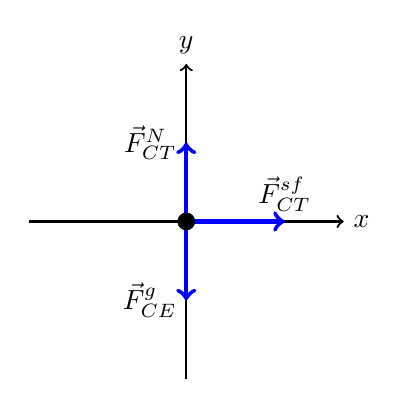
\begin{tikzpicture}
		\FBDaxes{0,0}{0}{axes}
		\FBDvectorXY{axes}{0,-1}{FG}
		\node[anchor=east] at (FGtip) {$\vec{F}^{g}_{CE}$};
		\FBDvectorXY{axes}{0,1}{FN}
		\node[anchor=east] at (FNtip) {$\vec{F}^{N}_{CT}$};
		\FBDvectorXY{axes}{1.25,0}{FSF}
		\node[anchor=south] at (FSFtip) {$\vec{F}^{sf}_{CT}$};
		\FBDdot{axes}
	\end{tikzpicture}
\end{center}
\textbf{Type of Friction} \\
The crate is not sliding against the roof of the truck (no relative motion), so any friction between it and the truck must be static. \\

\noindent\textbf{Direction of Friction} \\
For the crate to accelerate to the right, with the truck, the net force on it must also be to the right. Friction is the only horizontal force, so it must point to the right. If there were no friction, then the box would slide toward the back of the truck. Thus, the attempted relative motion would be to the left across the surface of the roof of the truck, and the force of static friction must oppose the attempted relative motion. \\

\noindent\textbf{Motion of the Truck} \\
If the ground is flat, then $\vec{a}=a\hat{x}$ (no vertical motion, which is assumed). We can see that
\begin{align*}
	F^{sf}_{CT} & = F^{net}_{x} = ma_{x} = ma, \\
	F^{N}_{CT} - F^{g}_{CE} & = F^{net}_{y} = ma_{y} = 0 \implies F^{N}_{CT} = F^{g}_{CE}.
\end{align*}
Furthermore, we know that
\[
F^{sf}_{CT} \leq \mu_{s} F^{N}_{CT} = \mu_{s}F^{g}_{CE} = \mu_{s}mg.
\]
Combined with the above observation that $F^{sf}_{CT} = ma$, we find that
\[
ma \leq \mu_{s}mg \implies a\leq\mu_{s}g.
\]
The acceleration of the truck must be less than $\mu_{s}g$ in order for the crate to not slide (the velocities of the crate and the truck are equal) relative to each other as the truck speeds up.
\end{TeacherMargin}
\begin{PresentSpace}
\vspace{-10pt}
\section*{S4-4: The Crate on Top of the Truck I (Gaining Speed)}
\vspace{-10pt}
\begin{itemize}
	\item A truck is initially moving to the right with speed $v_{i}$.
	\item The driver left a crate on top of the truck. We know the mass of the crate ($m_{c}$) and the coefficients of friction ($\mu_{s}$ and $\mu_{k}$).
	\item The truck begins \textit{speeding up}, but the driver wants to prevent the crate from sliding.
	\begin{itemize}
		\item Draw a free-body diagram for the crate.
		\begin{itemize}
			\item What kind of friction acts on it?
			\item What direction is the friction?
		\end{itemize}
		\item What do we know about the truck's \\
		velocity? What about its acceleration?
	\end{itemize}
\end{itemize}
\end{PresentSpace}
\begin{textblock*}{5cm}(22cm,5cm)
\centering
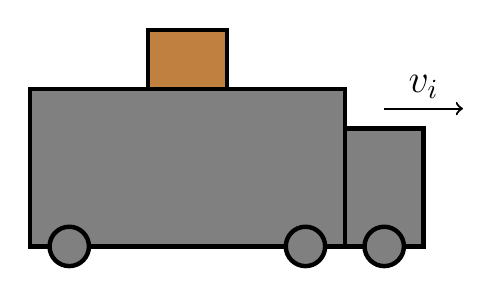
\begin{tikzpicture}
	\filldraw[ultra thick,color=black,fill=gray] (0,0) rectangle (4,2);
	\filldraw[ultra thick,color=black,fill=gray] (4,0) rectangle (5,1.5);
	\filldraw[ultra thick,color=black,fill=gray] (0.5,0) circle (0.25);
	\filldraw[ultra thick,color=black,fill=gray] (3.5,0) circle (0.25);
	\filldraw[ultra thick,color=black,fill=gray] (4.5,0) circle (0.25);
	\filldraw[ultra thick,color=black,fill=brown] (1.5,2) rectangle (2.5,2.75);
	\draw[thick,->] (4.5,1.75) -- (5,1.75) node[anchor=south] {\Large$v_{i}$} -- (5.5,1.75);
\end{tikzpicture}
\end{textblock*}
\newpage
\begin{TeacherMargin}
\begin{center}
	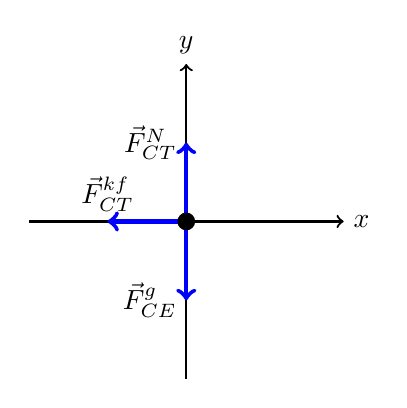
\begin{tikzpicture}
		\FBDaxes{0,0}{0}{axes}
		\FBDvectorXY{axes}{0,-1}{FG}
		\node[anchor=east] at (FGtip) {$\vec{F}^{g}_{CE}$};
		\FBDvectorXY{axes}{0,1}{FN}
		\node[anchor=east] at (FNtip) {$\vec{F}^{N}_{CT}$};
		\FBDvectorXY{axes}{-1,0}{FKF}
		\node[anchor=south] at (FKFtip) {$\vec{F}^{kf}_{CT}$};
		\FBDdot{axes}
	\end{tikzpicture}
\end{center}
\textbf{Differences} \\
The force of gravity doesn't change, and nor does the normal force that balances it out. The friction has switched directions and is now kinetic, rather than static. As the crate slides toward the front of the truck, its motion relative to the roof of the truck is also to the right, and the new direction of friction opposes this motion. \\

\noindent\textbf{Calculation}
We know $\vec{F}^{net} = m\vec{a}$, and therefore
\begin{align*}
	ma_{A} & = F^{net}_{x} = -F^{kf} & 0 & = F^{net}_{y} = F^{N} - F^{g},
\end{align*}
which means,
\begin{align*}
	a_{A} = -\frac{F^{kf}}{m} = -\mu_{kf} \frac{F^{N}}{m} = -\mu_{kf} \frac{F^{g}}{m} = -\mu_{kf} g. 
\end{align*}
\end{TeacherMargin}
\begin{PresentSpace}
\vspace{-10pt}
\section*{S4-5: The Crate on Top of the Truck II (Slamming on the Brakes)}
\vspace{-10pt}
\begin{itemize}
	\item A truck is initially moving to the right with speed $v_{i}$.
	\item We know the mass of the crate ($m_{c}$) and the coefficients of friction ($\mu_{s}$ and $\mu_{k}$).
	\item The driver suddenly has to slam on the brakes, causing the crate to begin sliding.
	\begin{itemize}
		\item Draw a free-body diagram for the crate.
		\begin{itemize}
			\item How is it different from before?
		\end{itemize}
		\item Determine the acceleration of the crate \\
		relative to the ground.
	\end{itemize}
\end{itemize}
\end{PresentSpace}
\begin{textblock*}{5cm}(22cm,5cm)
\centering
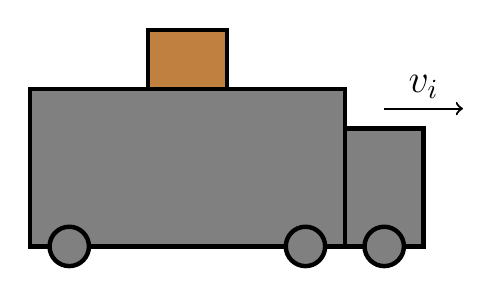
\begin{tikzpicture}
	\filldraw[ultra thick,color=black,fill=gray] (0,0) rectangle (4,2);
	\filldraw[ultra thick,color=black,fill=gray] (4,0) rectangle (5,1.5);
	\filldraw[ultra thick,color=black,fill=gray] (0.5,0) circle (0.25);
	\filldraw[ultra thick,color=black,fill=gray] (3.5,0) circle (0.25);
	\filldraw[ultra thick,color=black,fill=gray] (4.5,0) circle (0.25);
	\filldraw[ultra thick,color=black,fill=brown] (1.5,2) rectangle (2.5,2.75);
	\draw[thick,->] (4.5,1.75) -- (5,1.75) node[anchor=south] {\Large$v_{i}$} -- (5.5,1.75);
\end{tikzpicture}
\end{textblock*}
\newpage
\begin{TeacherMargin}

\end{TeacherMargin}
\begin{PresentSpace}
\vspace{-10pt}
\section*{Solving Problems Using Forces}
\vspace{-10pt}
\begin{itemize}
	\item Identify a system.
	\item Identify the (external) forces acting on the system.
	\begin{itemize}
		\item Draw a free-body diagram.
	\end{itemize}
	\item Identify the acceleration (\textbf{not a force}).
	\begin{itemize}
		\item Static/dynamic equilibrium (acceleration = 0)
		\item Dynamics (acceleration not 0)
	\end{itemize}
	\item Use the laws of motion.
\end{itemize}
\end{PresentSpace}
\newpage
\begin{TeacherMargin}

\end{TeacherMargin}
\begin{PresentSpace}
\section*{Main Ideas}
\begin{itemize}
	\item Forces arise from interactions between objects.
	\item There are many different \textit{kinds} of forces that we can analyze differently.
	\item Objects can only change their motion when acted upon by an external force.
	\item The net force on an object is equal to its mass times its acceleration.
	\item Forces are vectors.
	\item When more than one force acts on an object, we can add all the forces together.
	\item We can model forces quantitatively.
\end{itemize}
\end{PresentSpace}
\end{document}